\documentclass[a4paper]{article}

\usepackage[toc,page]{appendix}

\usepackage[spanish]{babel}
\usepackage[utf8]{inputenc}
\usepackage{amsmath}
\usepackage{graphicx}
\usepackage{fancyhdr}
\usepackage{amsmath}
\usepackage[colorinlistoftodos]{todonotes}
\usepackage{xcolor}
\usepackage{minted}
\usepackage[font=small,labelfont=bf]{caption}
\usepackage{enumitem}

\usepackage{hyperref}

\hypersetup{
    colorlinks,
    citecolor=blue,
    filecolor=blue,
    linkcolor=blue,
    urlcolor=blue
}

\newcommand*{\tabulardef}[3]{
  \begin{tabular}[t]{@{}lp{\dimexpr\linewidth-#1}@{}}
    #2&#3
\end{tabular}}

\usepackage{geometry}
\geometry{a4paper}

\begin{document}
\begin{figure}
\centering
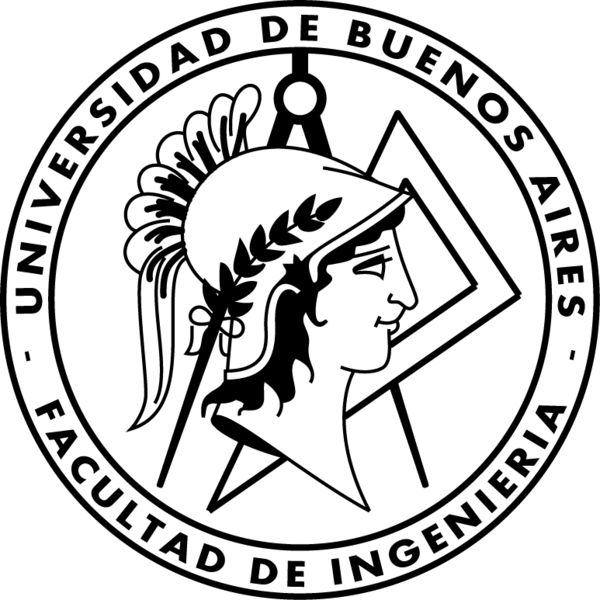
\includegraphics[scale=1]{./img/logo-facu}
\end{figure}

\title{\large\textsc{66.17 - Sistemas Digitales}\\
\large Trabajo Práctico Final - CORDIC}

\author{
Andrew Parlane \\
}

\maketitle

\newpage

\tableofcontents

\listoffigures

\newpage

\section{Introducción}

El objetivo de este trabajo es a diseñar, simular, verificar y sintetizar en FPGA un circuito digital que puede recibir coordenadas desde un PC, guardarles en memoria externa, rotarles usando un CORDIC 3D y dibujarles por una pantalla VGA.

El circuito digital debe funcionar con una Altera DE2 placa de desarrollo que tiene un cyclone II 2C35 FPGA.

\section{Herramientas}

Las herramientas que usé para este trabajo son:
\begin{itemize}[noitemsep]
\item Questa Sim v10.2c
\item Quartus II v13.0sp1
\item GNU Make v4.2.1
\item GCC v6.4.0
\item VGA Simulator \url{https://ericeastwood.com/lab/vga-simulator/}
\item MCUXpresso Config Tools v4.0
\item Kinetis Design Studio v3.2.0
\end{itemize}

\section{Elecciones del diseño}

\subsection{Memorias}

La elección más grande del diseño estuvo cual memoria usar para las coordenadas originales y la RAM de vídeo. La placa de desarrollo DE2 tiene tres memorias disponibles: \\

\begin{tabular}{| l | l | l | l |} \hline
\textbf{Tipo} & \textbf{Tamaño} & \textbf{velocidad máxima} & \textbf{Interfaz} \\ \hline
RAM de bloques & 52,5KB & 250MHz & Interna \\
SRAM & 512KB & 100MHz & Externa asíncrona 16 bit \\
SDRAM & 8MB & 143MHz & Externa sincronía 16 bit \\ \hline
\end{tabular} \\

El archivo de coordenadas dado tiene aproximadamente doce mil puntos. Si les guardamos con dos bytes cada componente, necesito 72KB. Elegí usar la SRAM porque no la RAM de bloques no es suficiente grande y la interfaz se pareció más sencillo que lo del SDRAM.

La resolución de vídeo especificado es 640x480 1 bit monocromo. Así la memoria de una cuadra es 37,5KB. Si quise tener un sistema de doble búfer habría necesitado una RAM de vídeo de 75KB que no entra en la RAM de bloques. El problema con usar RAM externa para vídeo con un sistema de doble búfer es que hay dos componentes que pueden accedan la memoria al mismo tiempo. Uno para leer los píxeles y uno para escribir los nuevos, así es necesario tener un árbitro. También el componente de VGA no puede esperar para leer, así tenía que ser un caché de al menos unos píxeles. El componente de transformación de coordenadas igual necesitaría una caché, o la habilidad de stall el pipeline.

Para evitar estos problemas decidí solo usar un búfer y elegí la RAM de bloques. Para prevenir errores en el display solo actualizo los píxeles durante el periodo de blanking vertical. En los temporización de VGA que uso hay 45 líneas de blanking vertical con un reloj de 25MHz, y el ancho de una línea es 800 píxeles. Ese me da 44000 píxeles o 1,44ms de blanking vertical. En ese tiempo tengo que borrar la cuadra anterior, y escribir la nueva. Si la RAM es direccionada por bit, solo puede borar un bit cada ciclo del reloj, y hay 307200 bits. Aun con un reloj de 250MHz duraría 1.2ms para borrar todo la RAM. Así elegí direccionar lo por byte. Con un reloj de 100MHz puede borrar todo en 0.4ms. Desafortunadamente ese significa que para escribir datos nuevos tengo que leer el byte corriente, encender el bit correcta, y escribirle. Pero aun si dura tres ciclos del reloj a 100MHz, puede escribir más de 33000 píxeles en el 1ms disponible. Solo tenemos 12000 coordenadas así esta diseño funciona bien.

\subsection{Formato de las coordenados}

El archivo de coordenados tiene los componentes entre -1.0 y 1.0 en ASCII. Tuve que elegir en que formato enviarles al FPGA, guardarles en SRAM y procesarles con el CORDIC. Elegí enviarles y guardarles en dos bytes cada componente. Ese es el ancho de bus de la SRAM. Usé punto fijo porque puedo usar operaciones rápidos de enteros y no necesito números muy largos o muy pequeños.

Las coordenadas son vectores donde cada componente puede estar entre -1.0 y 1.0. El largo máximo de un vector así es 1,73. La resolución de vídeo es 640x480, para que todos los píxeles entran en la pantalla, el offset máximo desde el centro es 240. Así tenemos que ampliar las coordenadas por un factor de aproximadamente 138. El algoritmo CORDIC tiene una ganancia de 1,64, porque usamos tres CORDICS, hay una ganancia total de 4,41. Nos deja una ganancia necesaria de aproximadamente 31. Elegí multiplicar cada componente por 29 antes de enviar les al FPGA. Ese significa que puedo sacar unos multiplicadores del circuito digital.

Ahora los datos están entre -29.0 y 29.0, así necesito seis bits por la parte entero y los otras 10 bits pueden ser por la parte fracional. Envié y guardo los datos en signed punto fijo Q\textsubscript{6.10}.

Después de la ganancia del CORDIC el valor estará entre -225 y 225 que necesita nueve bits de entero, así les pasa al CORDIC en signed punto fijo Q\textsubscript{9.23}.

\subsection{Velocidades de los Relojes}

La placa de desarrollo DE2 tiene un reloj de 50MHz. Para obtener la resolución de vídeo deseada a 60Hz necesito un reloj de 25MHz. Para actualizar la RAM de vídeo en el periodo de blanking vertical necesito al menos 74400 ciclos y tengo 1.44ms, así el reloj mínimo que puedo usar es 51.7MHz. Elegí usar uno de 100MHz, que es la velocidad máxima de la SRAM. Uso un PLL para generar los dos relojes necesarios.

\section{Implementación}

Dividí el proyecto en siete bloque mostrado en Figura \ref{fig:tp4_bloques}, algunos de eses bloques tienes bloques secundarios adentro los cuales voy a detallar más adelante.

\begin{figure}[!h]
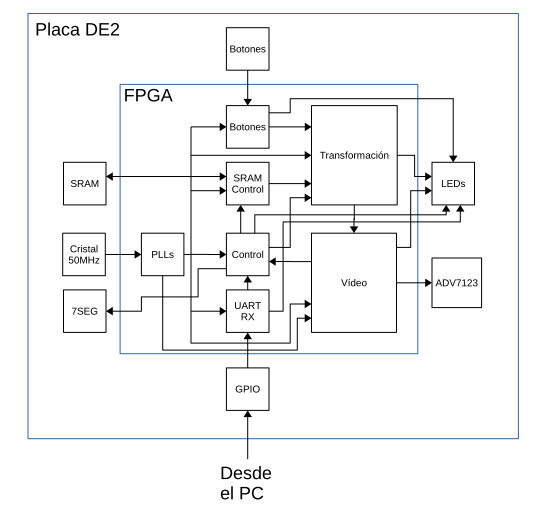
\includegraphics[width=15cm]{img/TP4_diagrama_de_bloques.png}
\captionof{figure}{Diagrama de Bloques del diseño completo.}
\label{fig:tp4_bloques}
\end{figure}

\subsection{Botones}

Ese componente toma los estados corrientes de los botones físicas y calcula los ángulos de rotaciones. Tiene un sincronizador para prevenir estados metastable, seis unidades de suma/resta y seis comparadores para guardar los valores entre 0 grados y 360 grados. Figura \ref{fig:botones} muestra cómo están conectados. Las señales mostrados ya están sincronizados al reloj.

\begin{figure}[!h]
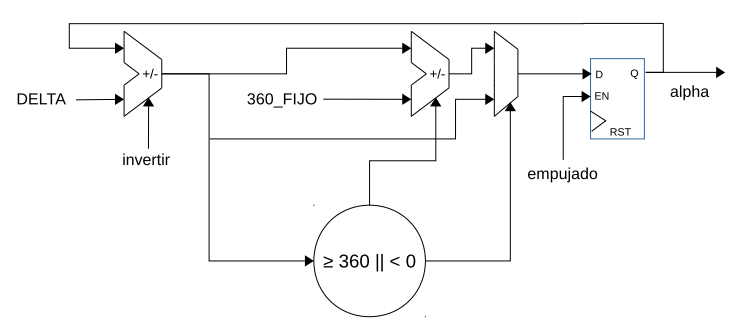
\includegraphics[width=15cm]{img/botones_bloques.png}
\captionof{figure}{Diagrama de Bloques de los botones.}
\label{fig:botones}
\end{figure}

\subsection{Controlador de SRAM}

La placa de desarrollo DE2 tiene una IS61LV25616AL-10T chip de SRAM, tiene un bus de direcciones de 18 bits y un bus bidireccional de datos de 16 bits, dando una memoria de 512KB. También hay varios líneas de \textit{enable}. Usé la hoja de datos para conocer cómo manejar las señales. Lecturas están fácil, cuándo el chip y la salida están activados el bus de datos es válido diez nanosegundos después de un cambio en el bus de direcciones, así puedo leer una palabra cada ciclo del reloj. Escrituras están un poco más complicados en que hay varias formas hacerles. A final elegí forma cuatro mostrado en Figura \ref{fig:sram_write}. La idea es activar el chip por diez nanosegundos y después desactivarle y dejarle diez nanosegundos más. En esta forma escrituras duran dos ciclos del reloj.

El diseño es muy sencillo, tiene un sicronizador para el bus de datos y un poco lógica para activar y desactivar las señales cómo querido.

\begin{figure}[!h]
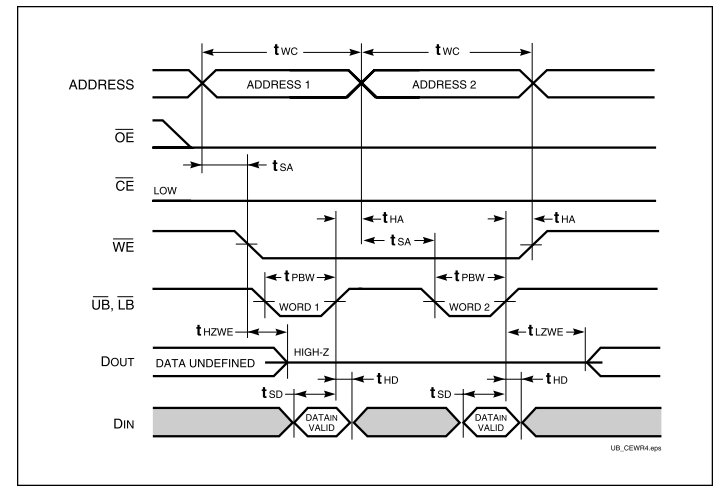
\includegraphics[width=15cm]{img/sram_write.png}
\captionof{figure}{Diagrama de temporización de escrituras a SRAM.}
\label{fig:sram_write}
\end{figure}

\subsection{PLLs}

No hay mucho decir sobre los PLLs. Usé el \textit{Quartus MegaWizzard} para generar un reloj de 100MHz y uno de 25MHz desde el reloj fuente de 50MHz.

\subsection {UART Rx}

Ese componente puede recibir y decodificar una señal UART. Paso la señal de entrada por un sincronizador y un anti-robote de cuatro bits. Después espera hasta hay un flanco descendente que significa el inicio de la trama. Comienza un contador para tomar una muestra en el medio de cada periodo de bit. Después de diez bits, comprueba que el bit de inicio es un cero y el bit de parada es un uno. Si no es un error de trama, o un break.

El componente toma dos genéricos, la cantidad de nanosegundos en el periodo del reloj, y la cantidad de nanosegundos en el periodo del bit. Les usa los dos para decidir cuando a tomar una muestra.

\subsection {Transformación}

Ese componente recibe los componentes de las coordenadas mientras están leídos de la SRAM. Hay una maquina de estados que conoce cual componente está recibiendo (X, Y o Z). Cuando recibe un componente lo extiende desde Q\textsubscript{6.10} a Q\textsubscript{9.23} y lo escribe al registro correspondiente. Cuando tiene todos los componentes del vector listo les pasa al CORDIC 3D.

Cuando el CORDIC 3D indica que un resultado es listo, convierte X y Y hasta la dirección y el bit de donde se queda el píxel en la RAM del vídeo, usa el formulario: $pixel = (y * 640) + x$ Los tres bits más bajos indican cual bit a encender, y los demás bits están la dirección. Esto lo hago sobre dos ciclos del reloj con un pipeline porque estuvo fallando el temporizado cuando intenté hacerle en un ciclo.

Dura tres ciclos del reloj a recibir todos los tres componentes de la coordenada, 30 ciclos por el CORDIC 3D y dos ciclos más para obtener la dirección y el bit del píxel. Eso es un total de 35 ciclos. El CORDIC 3D y la conversión hasta la dirección y bit son hecho con un pipeline, pero solo podríamos obtener un componente del vector cada ciclo desde la SRAM, así tiene un ancho de banda de 33,3MHz.

\subsection {CORDIC y CORDIC 3D}

El algoritmo básico de CORDIC en modo rotación es descrito con los formularios:

\[ x_{i+1} = x_i - y_i d_i 2^{-i} \]
\[ y_{i+1} = y_i + x_i d_i 2^{-i} \]
\[ \alpha_{i+1} = \alpha_i - d_i tg^{-1}(2^{-i}) \]

Donde $ d_i = -1 $ si $ z_i < 0 $ y $ d_i = 1 $ en otros casos. \\

Elegí implementar lo con un pipeline para obtener el mejor ancho de banda. Tengo una función que calcula todos los constantes de $ tg^{-1}(2^{-i}) $ por $ i = 0 $ hasta $ i = ETAPAS $ donde ETAPAS es un genérico.

\begin{figure}[!h]
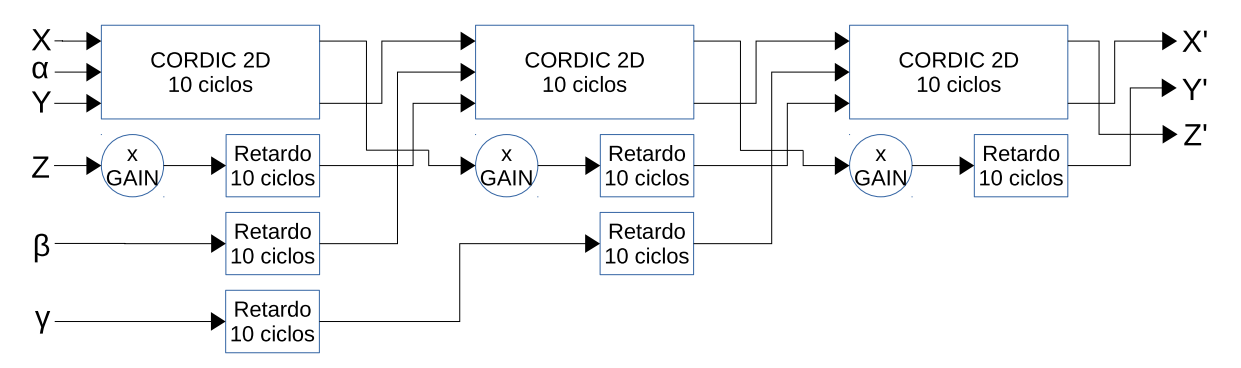
\includegraphics[width=15cm]{img/cordic3D_bloques.png}
\captionof{figure}{Diagrama de Bloques del CORDIC 3D.}
\label{fig:cordic3d}
\end{figure}

Mi implementación del CORDIC 3D es tres CORDICs normales en una cadena, como muestra figura \ref{fig:cordic3d}. Por cada CORDIC es necesario retardar los valores que no están usado en esa CORDIC. El algoritmo CORDIC tiene una ganancia de aproximadamente 1,64, y solo podríamos rotar dos componentes del vector cada vez. Así tenemos que multiplicar el componente que no es usado por esa ganancia. Calculo la ganancia exacto con una función que implementa la ecuación:

\[ A_n = \prod_{n} \sqrt{1 + 2^{-2i}} \]

\subsection{Subsistema de Vídeo}

El subsistema de Vídeo tiene unos bloques secundarios como mostrado en Figura \ref{fig:video_subsystem}. Hay la RAM de vídeo, el controlador de VGA por el DAC \textit{ADV7123} y unos bloques de lógica.

\begin{figure}[!h]
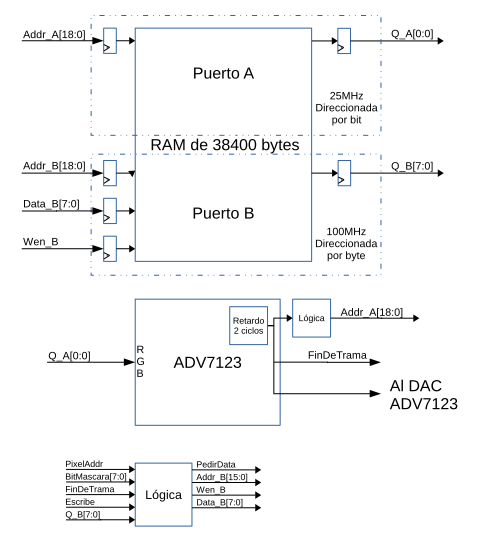
\includegraphics[width=15cm]{img/video_subsystem.png}
\captionof{figure}{Diagrama de Bloques del subsistema de vídeo.}
\label{fig:video_subsystem}
\end{figure}

Lo generé la RAM de vídeo con el Quartus MegaWizzard Tiene 38400 bytes y dos puertos cada uno con su propio reloj. Todos las entradas y salidas están registrados. Puerto A ejecuta a 25MHz, es direccionado por bit y solo es para lecturas. Puerto B ejecuta a 100MHz, es direccionado por byte y es lectura/escritura.

El controlador de VGA es el mismo que escribí para el Trabajo Práctico 2. Tiene salidas PixelX y PixelY que representan que pixel quieren: $ dir = (PixelY * ANCHO) + PixelX $. Porque la RAM de vídeo tiene registros en las entradas y salidas, dura dos ciclos del reloj obtener la data del píxel, así el ADV7123 retarda todos las otras señales para guardar todo sincronizado. También hay una salida FinDeTrama que indica cuando comienza el periodo de blanking vertical.

Cuando dispara la señal: FinDeTrama, comenzamos a escribir ceros por todo la RAM. Después de esto disparamos otra señal PedirData que va al bloque de Control comenzando el procesamiento de los vectores. Cuando termina con cada coordenada se da una dirección y una mascara de bit. Primero leemos el byte original, esa dura dos ciclos por los registros de entrada y salida, y en el tercer ciclo escribimos el OR del valor leído con la mascara de bit. Funciona bien, porque solo podríamos obtener valores nuevos del componente transformación cada tres ciclos.

Encontré un errata de silicio con las memorias de bloques con dos puertos usando relojes diferentes, donde unas escrituras pueden fallar. Por suerte había una solución alternativa cuando un puerto solo se usa para leer como en ese caso. Solo tuve que intercambiar puertas A y B.

\subsection{Control}

El bloque de Control es lo que junta todo, pero es muy sencillo. Hay una pequeña maquina de estados que desde reset espera por data desde el UART. La primer palabra es la cantidad de coordenadas que el PC va a enviar. Después cada palabra que lea, escribe al SRAM. Cuando ha recibido todos las coordenadas, cambia al estado de desocupación. Allá espera por la señal PedirData desde el subsistema de vídeo, y cambia al estado de transformación. Comienza a leer todos los datos de la SRAM y pasar al bloque de transformación. Cuando termina con esto devuelve al estado de desocupación. La maquina de estados es mostrado en Figura \ref{fig:control}.

\begin{figure}[!h]
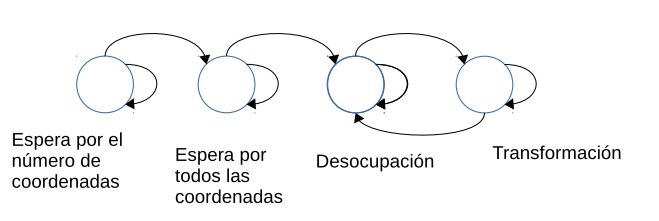
\includegraphics[width=15cm]{img/control.png}
\captionof{figure}{Diagrama de la maquina de estados del unidad Control.}
\label{fig:control}
\end{figure}

Además el bloque de control escribe el número de palabras esperado y el número recibido en los displays de siete segmentos.

\subsection{LEDs}

El estado corriente es mostrado por los LEDs. Hay dos LEDs verdes sobre cada botón, se encenden cuando el botón es empujado. Después uso cuatro LEDs rojos, les indican en orden de izquierda a derecha:

\begin{itemize}[noitemsep]
\item Error - Se enciende cuando escribimos a la RAM de vídeo durante la porción activo de la cuadra.
\item Estado de transformación - Se enciende cuando el bloque de control está en el estado de transformación. Porque entramos ese estado cada cuadra y hay casi 60 cuadras cada segundo, esa luz no enciende muy fuertemente.
\item Rx - Se enciende cuando el UART está recibiendo algo.
\item Estado de Rx - Se enciende cuando el bloque de control está esperando a data desde el PC.
\end{itemize}

\subsection {Programas de Apoyo en C}

Tuve que escribir algunos programas en C para varias razones.

\subsubsection{Manipulación de las coordenadas}

El archivo de coordenadas dado tiene todos los datos en ASCII. Sera posible enviarles así al FPGA pero no tiene sentido cuando una aplicación pequeña para la PC puede convertir los datos a un formato mejor. La aplicación \textit{parse\_coords} hace eso, lea el archivo dado y genera un archivo binario en little endian en el formato siguiente: \\

\begin{tabular}{ | r | r | l | } \hline
\textbf{Offset} & \textbf{Tamaño (bytes)} & \textbf{Descripción} \\ \hline
0 & 2 & Número de coordenadas \\
2 & 2 & Componente X del coordenada 0 \\
4 & 2 & Componente Y del coordenada 0 \\
6 & 2 & Componente Z del coordenada 0 \\
\multicolumn{1}{|r|}{...} & \multicolumn{1}{|r|}{...} & \multicolumn{1}{|c|}{...} \\ \hline
\end{tabular} \\

Cada componente es en el rango -29.0 a 29.0, y es en el formato de punto fijo Q\textsubscript{6.10}.

\subsubsection{Generación de Pruebas}

Para los bancos de pruebas del CORDIC, CORDIC 3D y la transformación necesité unos entradas y resultados esperado para comparar los resultados actual. Escribí un programa en C para generar un archivo de prueba. Ese no es ideal, me indica si hay un problema con mi implementación en VHDL pero no si hay un problema con mi comprehensión del algoritmo, pero es mejor que nada. Comprobé algunos resultados con un \href{https://g2384.github.io/work/cordic.html}{calculador de CORDIC en línea} para tener más confianza en el algoritmo.

El programa toma varios flags con cuales puedes controlar las pruebas generados. Los flags están detallados con el comando "./cordicTestGen --help":

\begin{minted}{bash}
Usage:
  cordicTestGen -h
  cordicTestGen -V
  cordicTestGen [options]
Options:
  -h, --help                Prints usage information.
  -V, --version             Prints version information.
  -n, --num_tests NUM       Number of tests to output.
  -3, --3d                  Generate a 3D cordic test file.
  -p, --gen_pixel_addr      Instead of the rotated cordic values, generate pixel address and bit mask.
  -r, --report_max          Write the max calculated value to stdout.
  -o, --output              Path to output file.

Examples:
  cordicTestGen -n 10000 -3 -o -
\end{minted}

Cuando ejecutas el programa, para cada línea de prueba genera tres valores aleatorios, un vector (X, Y) entre -29.0 y 29.0, y un ángulo: $ 0.0 \leq \alpha < 360.0 $. O en el caso del CORDIC 3D genera un vector (X, Y, Z) y tres ángulos. Todos están generado en punto fijo Q\textsubscript{9.23}.

\subsubsection{Convertador entre USB y UART}

Mi laptop no tiene un puerto de serial así tuve que encontrar otra forma enviar los datos al FPGA. Tengo una placa de desarrollo FRDM-K66F que tiene un procesador principal MK66FN2M0VMD18 y un coprocesador MK20DX128VFM5 ambos de NXP. El coprocesador tiene software de OpenSDA que conecta a un PC sobre USB y presenta varios interfaces. Uno de esas interfaces es un CDC para comunicaciones seriales. Así puedo enviar datos desde el PC sobre USB hasta el coprocesador que les convierta a UART y les envía al procesador principal.

Escribí un programa C pequeña para esa procesador principal que escucha por datos desde el PC y les envía al FPGA, usando un cable de ayuda desde un conector de GPIO del FRDM-K66F hasta un conector de GPIO del DE2.

\section{Simulación y Verificación}

Escribí bancos de pruebas para cada componente, en general intenté verificar el comportamiento usando \textit{SystemVerilog Asserts} por esa razón unos de las pruebas están escrito en \textit{SystemVerilog}.

Los bancos de pruebas de los componentes CORDIC, CORDIC 3D y transformación están basados en el banco de prueba que escribí por el sumador en el trabajo práctico 3, porque en todos casos tiene que leer unas entradas y resultados esperados y retardar los resultados esperados hasta el DUT da sus resultados. Encontré y arreglé varias bugs de mi implementación con estos bancos de pruebas. Figura \ref{fig:transform_waves} muestra las ondas del banco de prueba del componente transformación.

\begin{figure}[!h]
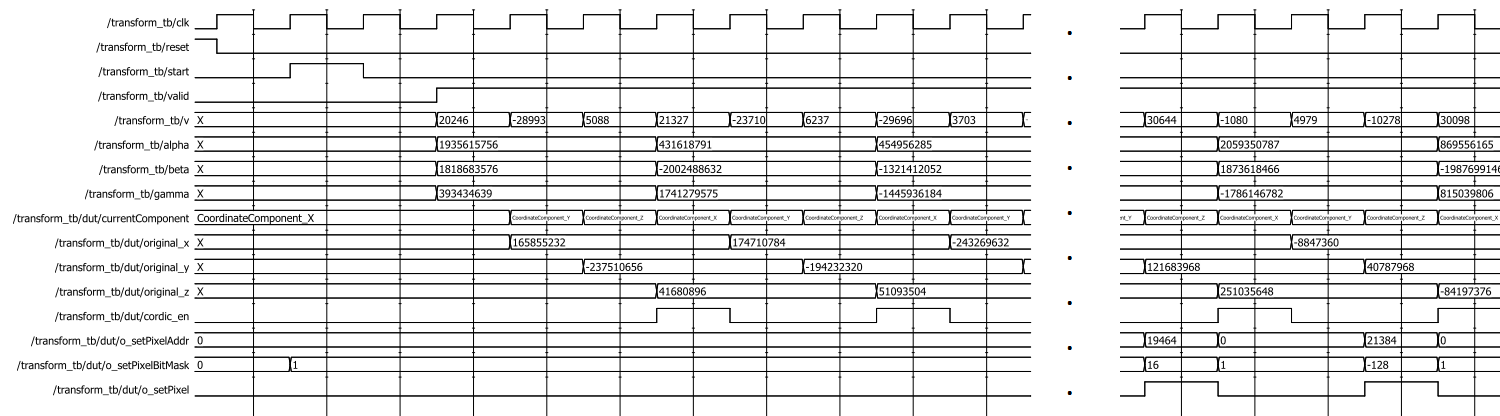
\includegraphics[width=15cm]{img/transform_waves.png}
\captionof{figure}{Ondas de la simulación del componente de transformación.}
\label{fig:transform_waves}
\end{figure}

\newpage
La salida del banco de prueba del componente uart\_rx es:

\begin{minted}{text}
# ---------------------------------------------------------------------------------
# Name                                      File(Line)                Failure Pass
#                                                                     Count   Count
# ---------------------------------------------------------------------------------
# /uart_rx_tb/inRst                         src/tb/uart_rx_tb.sv(148)       0    11
# /uart_rx_tb/recivingBecauseRxInFell       src/tb/uart_rx_tb.sv(157)       0     6
# /uart_rx_tb/rxInToReceiving               src/tb/uart_rx_tb.sv(166)       0     6
# /uart_rx_tb/rdDataValidWidth              src/tb/uart_rx_tb.sv(174)       0     3
# /uart_rx_tb/rdDataErrorWidth              src/tb/uart_rx_tb.sv(182)       0     2
# /uart_rx_tb/notErrorAndValid              src/tb/uart_rx_tb.sv(189)       0    11
# /uart_rx_tb/notBreakAndValidOrError       src/tb/uart_rx_tb.sv(197)       0    13
# /uart_rx_tb/rdDataValid                   src/tb/uart_rx_tb.sv(206)       0     3
# /uart_rx_tb/rdDataValidWhenExpectingError src/tb/uart_rx_tb.sv(214)       0     3
# /uart_rx_tb/rdDataErrorWhenExpectingValid src/tb/uart_rx_tb.sv(222)       0     2
# /uart_rx_tb/rdDataError                   src/tb/uart_rx_tb.sv(231)       0     2
# /uart_rx_tb/rdData                        src/tb/uart_rx_tb.sv(239)       0     3
# /uart_rx_tb/breakFallsWithReceiving       src/tb/uart_rx_tb.sv(247)       0     1
# /uart_rx_tb/breakDetect                   src/tb/uart_rx_tb.sv(256)       0     1
\end{minted}

La prueba de la RAM de vídeo no tiene asserts. Lo escribí como una prueba de concepto para verificar mi idea sobre la temporización del proceso de leer, ajustar y escribir los datos en tres ciclos del reloj. La prueba para el subsistema de vídeo es igual, el único diferencia es que tengo un programa de \textit{SystemVerilog} que captura las señales de VGA para uso con el \href{https://ericeastwood.com/lab/vga-simulator/}{simulador de VGA}. Figura \ref{fig:vga_sim} muestra el resultado de esa prueba que verifica que todas las señales están alineados bien.

\begin{figure}[!h]
\centering

\includegraphics[width=7cm]{img/vga_sim.png}
\captionof{figure}{Cuadra generado por el simulador de VGA desde señales de la prueba de la subsistema de vídeo.}
\label{fig:vga_sim}
\end{figure}

También escribí unas pruebas pequeñas para verificar el funcionamiento en el hardware actual. Lo hice para el controlador de SRAM porque aunque tuve confianza en mi comprehensión de la hoja de datos y mi implementación, estará posible que falta algo. También hice una prueba en FPGA para el UART Rx, más para verificar que mi código por el FRDM-K66F estuvo funcionando correctamente y que la conexión entre las dos placas estuvo bien.

\section{Síntesis}

He usado Quartus II para sintetizar el diseño, y escribir el bitstream al FPGA. Funciona la primera vez que le probé, que es una muestra de éxito de mis bancos de prueba. Hay un \href{https://www.youtube.com/watch?v=NT7cE3yvwjY}{vídeo de el diseño funcionando}, y figura \ref{fig:monitor} es un foto de la pantalla. Es más pequeño que planeaba y eso viene del manipulación de las coordenadas en el PC. La razón es que el largo máximo de un vector con cada componente entre -1.0 y 1.0 es aproximadamente 1,73, pero porque el modelo es una esfera cada vector tiene un largo de aproximadamente 1.0. Sera fácil cambiar el tamaño final, solo tendría que cambiar el factor de multiplicación en el programa \textit{parse\_coords} desde 29.0 hasta 50.0. También tendría que cambiar el código VHDL para conocer que los valores en SRAM son en Q\textsubscript{7.9} en vez de Q\textsubscript{6.10}. Una otra opción sera añadir dos multiplicadores en el componente de transformación a escalar los puntos. decidí dejar le por ahora, por si querría usar otras modelos que tal vez no serán esferas.

\begin{figure}[!h]
\centering
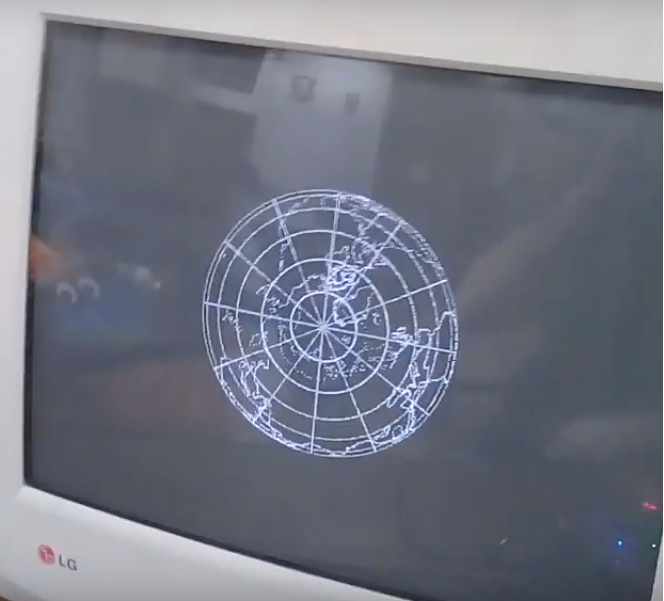
\includegraphics[width=7cm]{img/monitor.png}
\captionof{figure}{Foto de la pantalla mostrando el modelo del mundo.}
\label{fig:monitor}
\end{figure}

\subsection{Resumen de síntesis}
\begin{tabular}{| l | r | r | r|}
\hline
\textbf{Ítem} & \textbf{Utilizado} & \textbf{Disponible} & \textbf{Porcentaje Utilizado} \\ \hline
Logic Elements & 7.857 & 33.216 & 24\% \\
Registers & 3.196 & 33.216 & 23\% \\
Bits de memoria & 308.120 & 483.840 & 64\% \\
Global Clocks & 2 & 16 & 12,5\% \\ \hline
\end{tabular} \\

TimeQuest me da las frecuencias máximas de mis relojes: \\

\begin{tabular}{| l | r |}
\hline
\textbf{Reloj} & \textbf{Fmax} \\ \hline
clk25M & 99,72MHz \\
clk100M & 102,57MHz \\ \hline
\end{tabular} \\

\section{Código}

Todo el código es disponible en mi github: \url{https://github.com/andrewparlane/fiuba6617/tree/master/TP4}.

\end{document}
